\documentclass[10pt]{article}
\usepackage[preprint]{tmlr}
\usepackage{amsmath,amssymb,booktabs,graphicx,tabularx,longtable,array}
\usepackage[T1]{fontenc}
\usepackage{microtype}
\usepackage[hidelinks]{hyperref}
\usepackage{url}
\newcommand{\N}{12{,}769}
\newcommand{\JS}{D_{\mathrm{JS}}}
\newcommand{\MR}{D_{\mathrm{margin}}}
\newcommand{\suppref}[1]{Supplement, Section~#1}
\graphicspath{{figures/}}
\setlength{\emergencystretch}{1em}
\setlength{\LTcapwidth}{\textwidth}
\raggedbottom

\title{Sparse Circuit Families Across Grokking\\Supplementary Material}
\author{\name Alex Kolesnikov \\
\addr Lumiere Research Scholar Programme}
\renewcommand{\thesection}{S\arabic{section}}
\renewcommand{\thetable}{S\arabic{table}}
\renewcommand{\thefigure}{S\arabic{figure}}
\begin{document}
\maketitle
\section{Training and sampling}
The complete modular-addition domain consists of $113^2=12,769$ ordered pairs. A fixed pseudorandom partition gives 3,830 training and 8,939 test examples, shared by all five initialisations. Inputs have context length three, with a vocabulary of 114 tokens including the separator and an output vocabulary of 113 residue classes. Only final-position logits enter the task loss and circuit metrics. Models use TransformerLens, float32, one causal attention layer, residual width 128, four width-32 heads, 512 ReLU neurons, learned positional embeddings, no normalisation and no dropout. Full-batch AdamW uses learning rate 0.001, $(\beta_1,\beta_2)=(0.9,0.98)$, $\epsilon=10^{-8}$ and weight decay 1 for 40,000 steps. Checkpoints and metrics are saved every 50 steps.

Each run satisfies the eligibility rule: training accuracy reaches 99.9\%, a subsequent interval has test accuracy below 10\%, and test accuracy later reaches stable 99\% performance. Stable onset is the fifth checkpoint in the first sequence of five consecutive saved checkpoints reaching 99\% test accuracy. All models memorise by step 200. Table~\ref{tab:landmarks} gives their subsequent landmarks.
\begin{table}[h]
\centering
\caption{Full-model behavioural landmarks.}\label{tab:landmarks}
\begin{tabular}{crr}
\toprule Seed & First test accuracy $>10\%$ & Stable onset\\\midrule
0 & 1,550 & 5,900\\
1 & 3,450 & 9,050\\
2 & 4,600 & 7,750\\
3 & 6,950 & 10,400\\
4 & 3,600 & 6,850\\\bottomrule
\end{tabular}
\end{table}

The original plan used per-seed behavioural landmarks. Following pilot work, a common grid of seven steps was frozen before multi-seed circuit-family outcomes were available. It reproduces the pilot's full landmark grid: 200, 3,400, 7,450, 8,150, 8,500, 8,650 and 9,050. Delayed positions precede the first saved checkpoint above 10\% test accuracy; transitional positions lie between that point and stable onset. The grid has nine delayed, eleven transitional and fifteen stable positions. Seed~3's last analysed position is transitional, with test accuracy approximately 0.773. It is not reclassified or substituted with its later stable checkpoint.

\section{Masking and the original family search}
\label{sec:ssearch}
\subsection{Intervention and validation}
Components are indexed canonically as four whole attention heads and 512 individual MLP neurons. A head gate multiplies the complete head output before its residual-stream contribution. A neuron gate multiplies its post-ReLU activation before the MLP output projection. All positions use the same mask. Embeddings, positional embeddings, biases, unembeddings and other operations remain present. Retained weights are never retrained.

Validation at every analysed position checks that the all-retained mask reproduces full-model top-one predictions exactly and logits within numerical tolerance. Additional tests cover all-ablated and individual-component masks, component indexing, mask serialisation, repeat evaluation, hook restoration and parameter immutability. Fidelity is the integer prediction-agreement count divided by 12,769; displayed decimals do not determine eligibility.

\subsection{Candidate ranking and acceptance}
Let $g_i$ be a component's multiplicative gate. The ranking loss $L$ is mean cross-entropy against the full checkpoint's top-one predictions on the complete domain. Candidate deletion damage is estimated as $-g_i\partial L/\partial g_i$. Lower estimated damage is tested first in candidate batches of 16. The estimate ranks candidates only: each candidate undergoes an exact forward evaluation. The highest-fidelity admissible deletion in the first batch containing one is accepted, after which ranking is refreshed. A complete failed pass over every retained component establishes local single-deletion minimality.

For later members, let $r_i$ be the fraction of already accepted family masks retaining component $i$. At each ranking refresh, order the $n$ retained candidates by Taylor damage, breaking ties by canonical component index (heads first, then neurons). Assign ordinal percentiles $p_i=k_i/(n-1)$, with zero-based rank $k_i$; the singleton percentile is zero. Deletions are tested in ascending order of
\[
 s_i=p_i-0.5r_i.
\]
Thus a component reused in previous members is preferentially deleted. For the first member, no reuse transformation is applied: the original Taylor ranking is used directly. Ties in exact candidate fidelity are broken by canonical index.

The first requested member uses one path. Each later member allows restart indices 0--4, all starting from the full mask. Restart 0 orders by $(s_i,i)$. Other restarts permute candidates only within score groups of width $10^{-12}$ measured from each group's smallest score, not by chaining adjacent gaps. Groups remain ordered. Each ranking refresh recreates PCG64 with the same restart seed; no random initial mask is drawn. The seed is the unsigned big-endian integer formed from the first four SHA-256 bytes of the following UTF-8 string (indices are decimal; checkpoint and member indices are one-based):
\begin{quote}\small\ttfamily\raggedright
circuit-families|stage12-diversity-search|model\_seed=\{s\}|\allowbreak checkpoint\_index=\{t\}|\allowbreak family\_member\_index=\{c\}|\allowbreak restart\_index=\{r\}
\end{quote}
The displayed line breaks and spaces after them are not part of the seed material.

The Jaccard constraint is checked on the terminal candidate, not imposed on every intermediate deletion. A restart is accepted only if its endpoint meets fidelity, size and all pairwise-overlap constraints; the first such restart becomes the next member. The 10,000-exact-evaluation allowance for a requested member is shared sequentially across its restarts, not renewed for each one. The cell allowance is 50,000. A restart receives the smaller remaining allowance; failure to produce an admissible member ends the family search. The target is ten members. No original family reaches that target, so the observed six or seven members are not a saturation estimate.

\subsection{Complete top-one sensitivity accounting}
The family grid crosses six fidelity thresholds and three Jaccard ceilings at 35 positions. Of 630 executed cells, 300 are nonempty and 330 empty. Family sizes 0, 1, 2, 3, 4, 5, 6, 7 and 8 occur in 330, 3, 15, 34, 18, 15, 157, 48 and 10 cells respectively. All empty cells terminate on the first path at a locally minimal fidelity-valid mask larger than 258, using 531--6,757 evaluations (median 1,146). No empty result is imputed as a one-member family.

The first path's endpoint is identical across the three Jaccard ceilings because no previously accepted mask exists. Reconstruction therefore yields 210 unique endpoint rows, all locally single-deletion minimal and uncensored. Table~\ref{tab:e3grid} reports their size distributions and the number meeting the sparsity cutoff. Multiplying its position counts by three recovers the phase-by-fidelity nonempty-cell counts in the original 630-cell grid.
\begingroup\small\setlength{\tabcolsep}{4pt}
\begin{longtable}{r rr rr rr}
\caption{First greedy size by fidelity and phase. Size entries are minimum/median/maximum; sparse columns count positions at or below 258.}\label{tab:e3grid}\\
\toprule
Fidelity & Delayed size & Sparse & Transition size & Sparse & Stable size & Sparse \\

\midrule\endfirsthead
\toprule
Fidelity & Delayed size & Sparse & Transition size & Sparse & Stable size & Sparse \\

\midrule\endhead
\bottomrule\endfoot
0.800 & 483/490/496 & 0/9 & 76/383/478 & 4/11 & 39/47/64 & 15/15 \\
0.850 & 495/501/504 & 0/9 & 93/420/494 & 2/11 & 41/51/77 & 15/15 \\
0.900 & 504/507/510 & 0/9 & 118/473/508 & 2/11 & 44/54/82 & 15/15 \\
0.950 & 508/511/514 & 0/9 & 175/500/513 & 1/11 & 49/67/108 & 15/15 \\
0.975 & 510/514/515 & 0/9 & 246/512/515 & 1/11 & 59/72/119 & 15/15 \\
0.990 & 510/514/515 & 0/9 & 297/514/515 & 0/11 & 65/82/146 & 15/15 \\
\end{longtable}
\endgroup


At stable positions, the mean family count under $J\leq0.25$ is 3.6 at fidelity 0.800 and 4.4 at 0.990. The $J\leq0.50$ and $J\leq0.75$ conditions have identical means at each fidelity and reach 6.733 at 0.990. Separate searches need not return nested masks as fidelity changes. Nonemptiness itself cannot validate robustness to an overlap ceiling: the first mask is unaffected by that ceiling. The recovery of multiple members at $J\leq0.25$ is the relevant multiplicity check.

\section{Independent search and non-argmax criteria}
\subsection{Non-monotone optimisation and stopping}
Every stream begins with all 516 components retained. It selects deletion, addition or swap with weights 0.5, 0.1 and 0.4, sampling the eligible component sets uniformly. Exact complete-domain evaluation checks feasibility. Infeasible masks are rejected; feasible masks are accepted with probability $\min\{1,\exp(-\Delta|C|/T)\}$. Temperature declines geometrically from 0.5 to 0.02 as a function of unique exact stochastic evaluations. Evaluation results are cached by mask identity. The stochastic stage ends at 20,000 unique evaluations or 40,000 proposals.

The smallest verified mask then receives canonical-order cleanup: try each retained component, accept the first feasible deletion, restart the scan, and stop on a complete failed pass. Cleanup has its own 10,000-unique-evaluation allowance. Its completion proves local single-deletion minimality, not convergence of the stochastic search. The recorded \texttt{budget\_censored} flag is set when the proposal limit is reached or cleanup exhausts its budget. Reaching the planned 20,000-unique-evaluation allowance does not itself set this flag. A separate plateau flag records whether the best stochastic size remained unchanged for at least 5,000 unique evaluations. Table~\ref{tab:searchsummary} reports both: uncensored must not be read as plateau-converged.

\begingroup\small\setlength{\tabcolsep}{4pt}
\begin{longtable}{llrrrrr}
\caption{Annealing search outcomes. Size is minimum/median/maximum over streams. Censored and plateau are separate flags defined in Section S3.1. Every run completes local cleanup.}\label{tab:searchsummary}\\
\toprule
Criterion & Phase & Runs & Size & Sparse & Censored & Plateau \\

\midrule\endfirsthead
\toprule
Criterion & Phase & Runs & Size & Sparse & Censored & Plateau \\

\midrule\endhead
\bottomrule\endfoot
Top-one & Delayed & 90 & 508/514/515 & 0 & 86 & 42 \\
Top-one & Transition & 110 & 264/513/515 & 0 & 58 & 53 \\
Top-one & Stable & 150 & 58/71/136 & 150 & 0 & 43 \\
JS & Delayed & 90 & 509/513/515 & 0 & 90 & 35 \\
JS & Transition & 110 & 432/511/515 & 0 & 48 & 66 \\
JS & Stable & 150 & 209/276.5/368 & 40 & 0 & 21 \\
\end{longtable}
\endgroup


The post-review trace audit confirms that non-monotone moves were used. Stable top-one streams accept a median of 18 additions and 399 swaps; stable JS streams accept 24 additions and 424.5 swaps. They improve on the corresponding greedy endpoint in 137/150 and 58/150 cases. Delayed streams accept median additions/swaps of 54/78 for top-one and 70.5/65 for JS, with 40/90 and 60/90 improvements respectively. The optimiser therefore does more than repeat greedy deletion, although these moves remain restricted to feasible masks. All 150 stable streams for each criterion use the 20,000-unique-evaluation allowance; delayed top-one streams hit the proposal cap in 86/90 cases, and delayed JS streams in 90/90. Full per-stream and per-seed records accompany the audit.

Ten PCG64 streams are derived independently for each seed--checkpoint position, with SHA-256-based seeds binding the analysis and run identity. E5 streams also bind criterion and tolerance. The top-one positive control uses five streams at seed~0, step 9,050. Its gate requires at least four sparse successes and a best size no greater than 105, or 1.25 times the frozen greedy first-circuit size of 84. This gate passed before the 350-run E4 analysis.

\subsection{Metric definitions}
Jensen--Shannon divergence is the mean of the two KL terms to the midpoint distribution, as defined in the main paper, using natural logarithms and unscaled logits (temperature~1). Its frozen tolerance grid is $0.0001,0.0005,0.001,0.005,0.01,0.05$.

For margin preservation, let $y_x=\arg\max_k z_k(x)$ be the full checkpoint's predicted class and define
\[
 m(x)=z_{y_x}(x)-\max_{k\ne y_x}z_k(x),\qquad
 m_C(x)=z^C_{y_x}(x)-\max_{k\ne y_x}z^C_k(x).
\]
The masked margin uses the same reference class even if its own prediction differs. Normalised mean absolute reference-margin error is
\[
 \MR(C;M)=\frac{|X|^{-1}\sum_x|m_C(x)-m(x)|}
 {|X|^{-1}\sum_x|m(x)|}.
\]
Its frozen tolerances are $0.01,0.025,0.05,0.10,0.20,0.40$. Lower discrepancy is better for both criteria. The full-model reference margin is positive in these records; its scale is reported by checkpoint in Table~\ref{tab:positions}.

The deterministic grid retains the original top-one pseudo-target Taylor ranking, but accepts a deletion only when exact discrepancy meets the active tolerance; candidate selection within an admissible batch uses the discrepancy. Every one of the 420 planned runs is retained. Of these, 419 endpoints complete local cleanup and are uncensored. The exception is seed~0, step 9,050, margin tolerance 0.05: retained size 458, budget-censored and not locally minimal. Its observed endpoint remains in the grid and is marked in Table~\ref{tab:e5grid}.

\begingroup\small\setlength{\tabcolsep}{4pt}
\begin{longtable}{lr rr rr rr}
\caption{Complete deterministic non-argmax grid. Each phase reports minimum/median/maximum retained size and sparse positions. The starred group contains one censored endpoint (seed 0, step 9,050, size 458); all other endpoints are locally minimal and uncensored.}\label{tab:e5grid}\\
\toprule
Metric & Tolerance & Delayed & Sparse & Transition & Sparse & Stable & Sparse \\

\midrule\endfirsthead
\toprule
Metric & Tolerance & Delayed & Sparse & Transition & Sparse & Stable & Sparse \\

\midrule\endhead
\bottomrule\endfoot
JS & 0.0001 & 512/516/516 & 0/9 & 507/515/516 & 0/11 & 275/361/420 & 0/15 \\
JS & 0.0005 & 512/515/515 & 0/9 & 465/514/515 & 0/11 & 212/281/353 & 5/15 \\
JS & 0.001 & 510/514/515 & 0/9 & 455/511/515 & 0/11 & 194/254/323 & 9/15 \\
JS & 0.005 & 510/511/514 & 0/9 & 339/507/513 & 0/11 & 147/191/249 & 15/15 \\
JS & 0.01 & 508/510/512 & 0/9 & 304/499/510 & 0/11 & 132/170/217 & 15/15 \\
JS & 0.05 & 484/495/500 & 0/9 & 153/422/482 & 1/11 & 90/111/144 & 15/15 \\
Margin & 0.01 & 513/515/516 & 0/9 & 514/515/516 & 0/11 & 501/509/514 & 0/15 \\
Margin & 0.025 & 511/514/515 & 0/9 & 511/514/515 & 0/11 & 468/488/502 & 0/15 \\
Margin & 0.05 & 510/514/515 & 0/9 & 492/513/515 & 0/11 & 422/464/484$^{*}$ & 0/15 \\
Margin & 0.1 & 510/513/514 & 0/9 & 459/506/513 & 0/11 & 352/430/449 & 0/15 \\
Margin & 0.2 & 502/507/511 & 0/9 & 408/480/504 & 0/11 & 269/349/382 & 0/15 \\
Margin & 0.4 & 478/493/505 & 0/9 & 286/426/473 & 0/11 & 176/246/322 & 11/15 \\
\end{longtable}
\endgroup


\subsection{Stable-only calibration}
Before any E5 outcome, the design specified five streams at seed~0, step 9,050, for every frozen tolerance. A metric selects its strictest tolerance with at least four sparse successes, all five local cleanups complete, and no censored run. The 60 calibration runs are separate from the 350-stream full analysis. Table~\ref{tab:calibration} retains all tolerances, including failed gates. Jensen--Shannon selects 0.0005; no margin tolerance qualifies. In particular, 3/5 successes at margin tolerance 0.40 are not rounded up or replaced by its below-cutoff median.

\begingroup\small\setlength{\tabcolsep}{4pt}
\begin{longtable}{lrrrl}
\caption{All stable-only calibration results at seed 0, step 9,050. Every run is locally minimal and uncensored.}\label{tab:calibration}\\
\toprule
Metric & Tolerance & Min/median/max & Sparse & Gate \\

\midrule\endfirsthead
\toprule
Metric & Tolerance & Min/median/max & Sparse & Gate \\

\midrule\endhead
\bottomrule\endfoot
JS & 0.0001 & 284/290/294 & 0/5 & fail \\
JS & 0.0005 & 229/232/233 & 5/5 & pass; selected \\
JS & 0.001 & 209/211/214 & 5/5 & pass \\
JS & 0.005 & 160/162/167 & 5/5 & pass \\
JS & 0.01 & 140/142/144 & 5/5 & pass \\
JS & 0.05 & 96/101/103 & 5/5 & pass \\
Margin & 0.01 & 487/487/489 & 0/5 & fail \\
Margin & 0.025 & 458/462/462 & 0/5 & fail \\
Margin & 0.05 & 433/435/436 & 0/5 & fail \\
Margin & 0.1 & 396/398/399 & 0/5 & fail \\
Margin & 0.2 & 344/345/345 & 0/5 & fail \\
Margin & 0.4 & 253/256/260 & 3/5 & fail \\
\end{longtable}
\endgroup


\subsection{Checkpoint-level results}
Table~\ref{tab:positions} retains all 35 positions. E4 and E5 entries are minimum/median/maximum over ten streams. The full-model confidence scale and raw mean absolute margin error are given alongside E5. These quantities are diagnostics of the saved outputs, not an additional search or a fitted confidence adjustment. Per-run output distributions, discrepancies, accuracy and cross-entropy remain available in the machine-readable records.
\begingroup\small\setlength{\tabcolsep}{4pt}
\begin{longtable}{rrrrrrrr}
\caption{All checkpoint positions. G: greedy top-one size. A: annealing top-one size; JS: annealing Jensen--Shannon size at 0.0005 (both min/median/max). $m$: mean full-model reference margin; $e$: median raw mean absolute margin error among the ten JS endpoints. D/T/S indicate phase.}\label{tab:positions}\\
\toprule
Seed & Step & Phase & G & A & JS & $m$ & $e$ \\

\midrule\endfirsthead
\toprule
Seed & Step & Phase & G & A & JS & $m$ & $e$ \\

\midrule\endhead
\bottomrule\endfoot
0 & 200 & D & 513 & 512/512/512 & 513/513/513 & 2.71 & 0.03 \\
0 & 3400 & T & 515 & 515/515/515 & 512/512/512 & 4.16 & 0.12 \\
0 & 7450 & S & 77 & 70/73.5/77 & 270/274.5/287 & 12.80 & 4.02 \\
0 & 8150 & S & 82 & 70/75.5/81 & 302/307/313 & 11.51 & 3.11 \\
0 & 8500 & S & 75 & 65/69.5/71 & 316/320/322 & 11.06 & 2.67 \\
0 & 8650 & S & 70 & 64/66.5/71 & 287/291/294 & 12.72 & 4.05 \\
0 & 9050 & S & 84 & 63/66/68 & 229/232/234 & 16.22 & 7.50 \\
1 & 200 & D & 515 & 514/514/514 & 515/515/515 & 2.70 & 0.02 \\
1 & 3400 & D & 515 & 515/515/515 & 515/515/515 & 4.69 & 0.07 \\
1 & 7450 & T & 515 & 515/515/515 & 515/515/515 & 5.20 & 0.07 \\
1 & 8150 & T & 514 & 512/512/512 & 512/512/512 & 6.57 & 0.16 \\
1 & 8500 & T & 511 & 503/505/506 & 506/506/506 & 5.60 & 0.17 \\
1 & 8650 & T & 493 & 468/473.5/479 & 495/495/497 & 7.59 & 0.27 \\
1 & 9050 & S & 146 & 115/127/136 & 261/266.5/273 & 13.32 & 3.18 \\
2 & 200 & D & 513 & 511/511/511 & 512/512/512 & 2.61 & 0.03 \\
2 & 3400 & D & 515 & 515/515/515 & 515/515/515 & 4.97 & 0.08 \\
2 & 7450 & T & 297 & 264/278.5/291 & 432/434/443 & 10.75 & 0.76 \\
2 & 8150 & S & 105 & 97/107/112 & 343/346.5/356 & 7.66 & 0.83 \\
2 & 8500 & S & 87 & 81/84.5/87 & 293/297.5/303 & 10.90 & 2.85 \\
2 & 8650 & S & 93 & 76/82/86 & 267/273/277 & 12.47 & 4.28 \\
2 & 9050 & S & 92 & 65/70/72 & 209/217/221 & 15.73 & 7.61 \\
3 & 200 & D & 510 & 508/508/508 & 509/509/509 & 2.54 & 0.04 \\
3 & 3400 & D & 514 & 514/514/514 & 513/513/513 & 4.54 & 0.12 \\
3 & 7450 & T & 515 & 515/515/515 & 515/515/515 & 5.43 & 0.08 \\
3 & 8150 & T & 515 & 514/514/514 & 511/511/511 & 3.05 & 0.10 \\
3 & 8500 & T & 515 & 514/514/514 & 512/512/512 & 4.41 & 0.12 \\
3 & 8650 & T & 514 & 513/513/513 & 511/511/511 & 5.44 & 0.14 \\
3 & 9050 & T & 509 & 494/496/498 & 502/503/503 & 9.19 & 0.24 \\
4 & 200 & D & 513 & 513/513/513 & 514/514/514 & 2.64 & 0.04 \\
4 & 3400 & D & 515 & 515/515/515 & 513/513/513 & 4.73 & 0.11 \\
4 & 7450 & S & 89 & 73/77/79 & 235/239/244 & 13.75 & 5.62 \\
4 & 8150 & S & 72 & 66/69.5/74 & 359/360.5/368 & 8.91 & 1.64 \\
4 & 8500 & S & 67 & 60/63/66 & 288/291/293 & 12.49 & 4.50 \\
4 & 8650 & S & 65 & 58/60.5/64 & 261/265/268 & 13.94 & 5.91 \\
4 & 9050 & S & 74 & 61/64/69 & 223/226.5/232 & 16.51 & 8.49 \\
\end{longtable}
\endgroup


\section{Analysis sequence and provenance}
The original protocol was initiated before family results and later amended to the common checkpoint grid before the multi-seed family analysis. The original analysis was frozen after its independent reproduction and downstream revalidation. The five follow-ups do not replace that freeze:
\begin{enumerate}
\item E1 compares the final stable pairs with matched overlap nulls; E2 evaluates matched random masks; E3 reconstructs first-path endpoints from existing records. These were designed after the original results were visible.
\item The E4--E5 robustness contract was committed before any E4 checkpoint search. It fixed the 35 positions, continuous retained-size endpoint, non-monotone optimiser and budgets, stable positive-control gate, and both E5 metric grids.
\item After E4 completed but before E5 ran, an amendment added metric-specific stable calibration and full annealing at the selected tolerances. The deterministic grids remained required for both metrics.
\item Calibration passed for Jensen--Shannon and failed for margin. An implementation initially required both metrics to pass. After calibration, that execution check was corrected to follow the already-written per-metric eligibility rule. No tolerance, gate or result changed. The full Jensen--Shannon analysis ran; the full margin analysis did not.
\end{enumerate}
No delayed or transitional E5 outcome selected the Jensen--Shannon tolerance. Nevertheless, that tolerance is calibrated for compact recovery at one stable position, rather than a task-independent notion of equal fidelity. Its checkpoint-to-checkpoint behaviour is consequently reported together with the full tolerance grids.

Source configurations, masks and results retain their original manifests. A separately recorded post-review follow-up audits those outputs and performs the fixed-mask evaluations in S7; it changes no E1--E5 configuration or result. The manuscript builder, \texttt{build\_manuscript.py}, only aggregates completed tables. It records input hashes in \texttt{source\_registry.json}, validates coverage and key numerical claims, and exports display data. The accompanying README gives build instructions and a source map. Exact-domain evaluation removes input-sampling uncertainty in a mask's reported fidelity, not variability across training seeds or search paths.

\section{Matched structural and behavioural nulls}
\subsection{Exact Jaccard null}
For two independently sampled subsets of an $N$-component universe with fixed sizes $a$ and $b$, intersection $K$ has probability
\[
 \Pr(K=k)=\frac{\binom{a}{k}\binom{N-a}{b-k}}{\binom{N}{b}},
 \quad \max(0,a+b-N)\leq k\leq\min(a,b).
\]
Jaccard is $K/(a+b-K)$. Its expectation is calculated by summing this transform against the exact distribution; substituting the mean intersection into the ratio is not the same calculation. The composition-matched null draws independently within the four-head and 512-neuron strata. Its intersection law is the convolution of the two hypergeometric laws. Since every observed final circuit retains all four heads, the stratified null always shares those heads.

The analysis covers 78 within-family pairs from seeds 0, 1, 2 and 4 at step 9,050, with 100,000 deterministic Monte Carlo draws per pair and null as a numerical check. Each row records the exact mean, standard deviation, equal-tail 95\% null interval, inclusive lower and upper tails, mid-percentile and z-score, alongside simulation summaries. The interval describes random-mask Jaccard variation, not uncertainty in an estimated scientific effect. The pooled median z-scores are +2.37 for size matching and +1.67 for composition matching. Seed~1 is closer to its matched expectation than the other final stable seeds. Pair rows share masks and are not independent hypothesis tests.

\begin{figure}[tb]
\centering
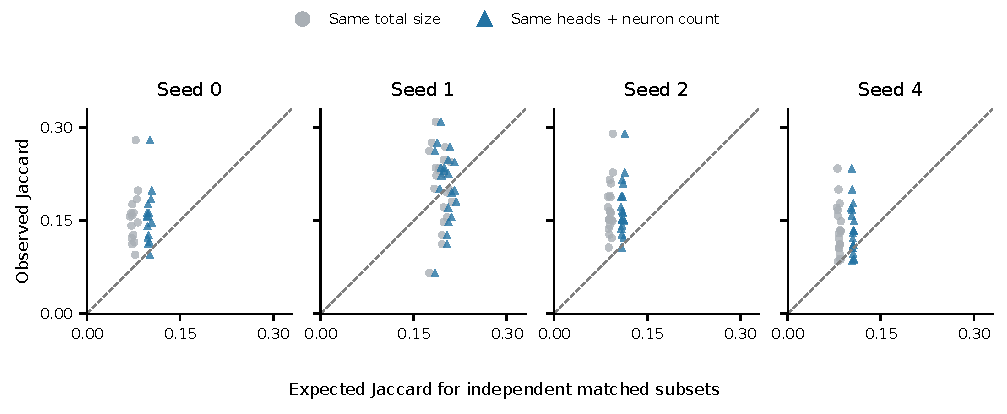
\includegraphics[width=\linewidth]{overlap_nulls.pdf}
\caption{\textbf{Small raw overlaps exceed the matched random-subset expectation in aggregate.} The 78 final within-family pairs, separated by model. Each pair is plotted against its exact expected Jaccard under two matching rules. Points above the diagonal overlap more than their matched expectation. Seed~1 lies closer to equality than the other models. The two marks for a pair share the same observed value; they are alternative baselines, not additional observations.}
\label{fig:overlap}
\end{figure}

\subsection{Behavioural null}
The 27 observed masks give 21 unique seed/head-count/neuron-count profiles. For each, 100 total-size-matched and 100 composition-matched masks are evaluated over the full domain. Matching by profile avoids treating duplicate profiles as independent random-mask samples. Seeds are derived from canonical SHA-256 material including the analysis, checkpoint, composition and null identity; PCG64 draws are deterministic.

No random mask passes the 0.990 threshold. Each profile/null has zero successes in 100 draws, yielding a two-sided exact 95\% upper confidence limit of 0.0362 for its random-mask pass probability. The plus-one Monte Carlo tail $1/101$ is not a selection-corrected significance test: the observed masks were selected by optimisation, whereas the null masks were sampled uniformly. Neither null preserves empirical component-selection frequencies or reproduces the family-search selection process.

\section{Original secondary analyses}
\subsection{Final family structure and operand profiles}
At step 9,050, seeds 0, 1, 2 and 4 contribute respectively 6, 7, 7 and 7 primary circuits. Their retained-size ranges are 66--84, 146--180, 81--92 and 74--82; median sizes are 71, 169, 85 and 80. Within-family Jaccard ranges are 0.0949--0.2797, 0.0657--0.3092, 0.1067--0.2899 and 0.0845--0.2339. The full 78-pair listings are retained rather than reduced to the most separated example.

Q1--Q4 partition the test split by low (0--56) and high (57--112) operands. Q1 uses two low operands; Q2 low/high; Q3 high/low; Q4 two high operands. The four subset fidelities form a profile, and pair distance is the maximum absolute coordinate difference. Deterministic complete linkage at tolerance 0.05 defines profile groups. These subsets are unseen in model training but included in the complete-domain circuit-discovery objective.

All fifteen stable primary families form one group. Across the final 78 pairs, profile distances range from 0.000616 to 0.007653, with median 0.003133. Across all stable primary families, the maximum is 0.009885. Among the 300 nonempty sensitivity cells, 285 form one group and 15 form two; all two-group outcomes occur at fidelity 0.800, 0.850 or 0.900. No higher-fidelity setting yields two groups at the selected tolerance.

An exploratory seed~1 analysis discovers one circuit separately on each operand subset and evaluates all sixteen discovery-by-evaluation combinations. Mean diagonal fidelity is 0.99021 and mean off-diagonal fidelity 0.88420; Q1-to-Q4 transfer is 0.66709. This different discovery objective reveals conditional asymmetry without establishing distinct algorithms.

\subsection{Fourier pilot}
At seed~1, step 9,050, centred full-domain output logits are Fourier transformed. The diagnostic asks whether the correct shifted-addition relation ranks first and accounts for at least half of non-DC power. The full model and one sparse circuit at each of six fidelity thresholds pass. Circuit addition-manifold fractions range from 0.691749 to 0.731648. The primary pilot circuit retains 146 components, with fidelity 0.990054 and addition-manifold fraction 0.731648. This diagnostic does not cover all final family members.

\subsection{Matched longitudinal comparisons and original endpoints}
For every earlier--later checkpoint pair within a seed, fidelity matching pairs circuits within 0.01 global agreement and size matching pairs circuits within five components. Both use one-to-one matching without replacement, first maximising pair count and then minimising total matching discrepancy. Of 105 possible within-seed checkpoint comparisons per scheme, 26 admit fidelity matches and 22 size matches. Comparisons lacking eligible circuits remain undefined.

The original primary family-size change from step 200 to 9,050 is $+6,+7,+7,0,+7$, with median +7, mean +5.4 and exact two-sided sign-test probability 0.125 after omitting the zero difference. Step 3,400 to 9,050 gives the same values, not independent evidence. The originally specified change in transfer-group count is undefined because the early families are empty; no group count is imputed as zero. Secondary matched comparisons do not show a consistent cross-seed contraction towards a single mask and are retained as descriptive records, not a new confirmatory endpoint.

\subsection{Controls}
One random-label model uses the same inputs and split with a separately seeded permutation of the complete label vector. No primary family is recovered at any of the seven steps. A structured no-generalisation control was unavailable under its prespecified eligibility rule and was not replaced post hoc. These controls do not isolate the effect of generalisation from task structure or correlated training dynamics.

\section{Post-review saved-mask and search audit}
\label{sec:reviewfollowup}
This exploratory follow-up was specified after the peer review, with the evaluation protocol and implementation committed before new masked forward evaluations. It uses the original 27 final masks and checkpoints authenticated by E1/E2, not new searches or replacements selected for favourable diagnostics. SHA-256 hashes identify the original mask files, dataset, checkpoints, builder, protocol and outputs. The evaluation reproduces every stored original agreement count and JS value (absolute tolerance $2\times10^{-7}$), checks full-mask logits, and verifies unchanged weights and restored hooks. Seventy logical evaluations include four full masks, four attention-only masks, four cores, four unions, 27 members and 27 core-removed members. Computation is deterministic on CPU with float32 model arithmetic and float64 diagnostic reductions; identical masks may reuse computation while retaining separate labelled records.

\subsection{Families in independently generated mask pools}
The audit uses all 350 E4 runs and all 350 full JS runs. At each of the fifteen stable positions it computes all 45 pairwise overlaps among ten endpoints. A mask is eligible if it satisfies the run's active fidelity criterion and retains at most 258 components. Exhaustive enumeration of subsets identifies the largest family at Jaccard 0.25 and 0.50, with deterministic lexicographic selection among tied subsets. This is an exact maximum within the saved ten-mask pool, not within all possible masks. Duplicate masks cannot enlarge a family. No overlap term entered either annealing objective. Table~\ref{tab:savedfamilies} reports all stable models; the pairwise file retains every pair rather than only selected compatible pairs.
\begingroup\small\setlength{\tabcolsep}{4pt}
\begin{longtable}{lrrrrr}
\caption{Largest qualifying family in each pool of ten saved annealing masks, computed exactly after the runs. Ranges span stable positions within a seed. Multiplicity means at least two qualifying masks at Jaccard 0.50; zero means no mask meets the 258-component bound.}\label{tab:savedfamilies}\\
\toprule
Criterion & Seed & Positions & $J\leq0.25$ & $J\leq0.50$ & Multiplicity \\

\midrule\endfirsthead
\toprule
Criterion & Seed & Positions & $J\leq0.25$ & $J\leq0.50$ & Multiplicity \\

\midrule\endhead
\bottomrule\endfoot
Top-one & 0 & 5 & 7--10 & 10--10 & 5 \\
Top-one & 1 & 1 & 1--1 & 10--10 & 1 \\
Top-one & 2 & 4 & 2--10 & 10--10 & 4 \\
Top-one & 4 & 5 & 10--10 & 10--10 & 5 \\
JS & 0 & 5 & 0--1 & 0--10 & 1 \\
JS & 1 & 1 & 0--0 & 0--0 & 0 \\
JS & 2 & 4 & 0--1 & 0--10 & 1 \\
JS & 4 & 5 & 0--1 & 0--10 & 2 \\
\end{longtable}
\endgroup


\subsection{Shared and alternative neurons}
Write each original member as $C_j=H\cup N_j$, where $H$ is the set of four heads. For each seed, define $K=\bigcap_j N_j$ and $V=\bigcup_j N_j$. The interventions retain $H$, $H\cup K$, $H\cup V$, and $H\cup(N_j\setminus K)$, in addition to each original member and the full model. No retained weight is changed. Attention-only fidelity is 0.0165--0.0367; core fidelity is 0.0324--0.0458. The common-neuron counts are 3, 8, 4 and 1, so none is an empty-intersection no-op. All core-removed members fail 0.990. This establishes a collective contribution of the shared set in each tested member, not necessity of each neuron individually or of that set in every possible faithful mask.

Unions retain 283, 500, 339 and 361 total components and attain fidelity 0.9829, 0.9995, 0.8599 and 0.8541 respectively. Their failures show that fidelity need not increase when components are restored. The tested common core is the literal all-member intersection; this experiment does not search for an approximately shared sufficient core or perform causal interchange between representations.

\subsection{Same-mask cross-metric and confidence diagnostics}
For the same full and masked logits, JS is recomputed at common temperatures 1, 2 and 4. Temperature changes neither weights nor argmax decisions. The output records mean, median, 95th and 99th percentiles and maximum divergence, all six frozen JS and margin threshold decisions at temperature 1, train/test agreement and accuracy, and subdivisions by whether the full model is correct. Per-input arrays retain reference and masked predictions, labels, margins and JS values. Centred-logit error subtracts each input's mean across output classes, computes global RMSE, and divides by the full model's centred-logit RMS; this removes the irrelevant common logit offset. A zero normaliser is recorded as undefined. Table~\ref{tab:originalmetrics} shows ranges for the original members. Their relative centred-logit RMSE is 0.560--0.841, consistent with substantial changes beyond the winning class.
\begingroup\small\setlength{\tabcolsep}{4pt}
\begin{longtable}{rrrrrr}
\caption{Cross-metric scores of the same 27 original family masks at step 9,050. Ranges across members; JS uses natural logs. Both reference and masked logits use the stated common temperature. Margin error is normalised by the reference margin.}\label{tab:originalmetrics}\\
\toprule
Seed & $n$ & JS, $T=1$ & JS, $T=2$ & JS, $T=4$ & Margin error \\

\midrule\endfirsthead
\toprule
Seed & $n$ & JS, $T=1$ & JS, $T=2$ & JS, $T=4$ & Margin error \\

\midrule\endhead
\bottomrule\endfoot
0 & 6 & 0.128--0.213 & 0.379--0.463 & 0.450--0.487 & 0.852--0.884 \\
1 & 7 & 0.025--0.028 & 0.116--0.126 & 0.218--0.230 & 0.653--0.668 \\
2 & 7 & 0.108--0.140 & 0.335--0.382 & 0.415--0.442 & 0.848--0.863 \\
4 & 7 & 0.169--0.185 & 0.413--0.430 & 0.466--0.475 & 0.880--0.889 \\
\end{longtable}
\endgroup


Across all fifteen stable positions, the descriptive Spearman correlation between mean full-model reference margin and median JS-annealing size is $-0.949$. Within seeds 0, 2 and 4 it is $-1.00,-1.00,-0.90$, from five, four and five positions; seed~1 has one. The export also retains all 35 positions and pooled/within-seed correlations. No independent-sample significance test is attached to nested checkpoints. The fixed-mask temperature diagnostic is not a temperature-controlled search and does not establish a confidence-independent compression effect.

\end{document}
